%
% ---------------------------------------------------------------
% Copyright (C) 2012-2018 Gang Li
% ---------------------------------------------------------------
%
% This work is the default powerdot-tuliplab style test file and may be
% distributed and/or modified under the conditions of the LaTeX Project Public
% License, either version 1.3 of this license or (at your option) any later
% version. The latest version of this license is in
% http://www.latex-project.org/lppl.txt and version 1.3 or later is part of all
% distributions of LaTeX version 2003/12/01 or later.
%
% This work has the LPPL maintenance status "maintained".
%
% This Current Maintainer of this work is Gang Li.
%
%

\documentclass[
 size=12pt,
 paper=smartboard, %a4paper, smartboard, screen
 mode=present, %present, handout, print
 display=slides, % slidesnotes, notes, slides
% nohandoutpagebreaks,
% pauseslide,
style=tuliplab,
% nopagebreaks,clock
% hlentries=true,
% hlsections = true,
pauseslide,
fleqn,leqno]{powerdot}

\hypersetup{pdfpagemode=FullScreen}
% \usepackage[toc,highlight,blackslide,slidesonly,sounds,HA]{HA-prosper}
\usepackage{amssymb}
\usepackage{amsmath}
\usepackage{rotating}
\usepackage{graphicx}
\usepackage{boxedminipage}
\usepackage{media9}
\usepackage{rotate}
\usepackage{calc}
\usepackage[absolute]{textpos}
\usepackage{psfrag,overpic}
\usepackage{fouriernc}
\usepackage{pstricks,pst-node,pst-text,pst-3d,pst-grad}
\usepackage{moreverb,epsfig,color,subfigure}
\usepackage{color}
\usepackage{pstricks}
\usepackage{pstricks-add}
\usepackage{pst-text}
\usepackage{pst-node, pst-tree}
\usepackage{booktabs}
\usepackage{etex}
\usepackage{breqn}
\usepackage{multirow}
\usepackage{gitinfo2}


\usepackage{listings}
\lstset{frameround=fttt,
frame=trBL,
stringstyle=\ttfamily,
backgroundcolor=\color{yellow!20},
basicstyle=\footnotesize\ttfamily}
\lstnewenvironment{code}{
\lstset{frame=single,escapeinside=`',
backgroundcolor=\color{yellow!20},
basicstyle=\footnotesize\ttfamily}
}{}


\usepackage{fouriernc}
\usepackage{hyperref}

%%%%%%%%%%%%%%%%%%%%%%%%%%%%%%%%%%%%%%%%%%%%%%%%%%%%%%%%%%%%%%%%%%%%%%%%
% title
% TODO: Customize to your Own Title, Name, Address
%
\title{Identifying Customers
}
\author{
Xichen Tang
\\
QUT
% \href{mailto:gangli@acm.org}{gangli@acm.org}
% \and % more authors
}
\date{\today}



% Customize the setting of slides
\pdsetup{
% theslide=\arabic{slide}~/~\pageref*{lastslide},
% theslide=\arabic{slide},
rf=\href{http://www.tulip.org.au/members}{
Last Changed by: \textsc{Xichen Tang}\  (\today)
},
cf=\hyperlink{blankslide}{Identifying Customers},
trans=Fade,
list={labelsep=1em,leftmargin=*,itemsep=0pt,topsep=5pt,parsep=0pt},
% counters={theorem,lemma},
% randomdots,dmaxdots=80
}


\begin{document}

\maketitle
\section{Directory}
\begin{slide}[toc=,bm=]{Introduce}
\tableofcontents[content=sections,type=1]
\end{slide}
\section{Subject Introduce}
\begin{slide}[toc=,bm=]{Introduce}
\begin{itemize}
\item The kaggle subject:Santander Customer Transaction Prediction

\end{itemize}
In this challenge, we need to identify which customers will make a specific transaction in the future, irrespective of the amount of money transacted.
\includegraphics[width=6in]{face}
\end{slide}
\begin{slide}{Data}
\begin{itemize}
    \item train_data
\end{itemize}

\begin{tabular}{|c|c|c|c|c|c|c|}%一个c表示有一列,格式为居中显示(center)

ID_code&target&var_0&var_1&...&var_198&var_199\\%第一行第一列和第二列  中间用&连接
 \hline
train_0&0&8.9255 &-6.7863 &...  & 12.7803 & -1.0914  \\
 \hline
train_1&0&11.5006& -4.1473 &...  &18.3560  &   1.9518\\
\end{tabular}
\begin{itemize}
\item test.csv
\end{itemize}

\begin{tabular}{|c|c|c|c|c|c|}%一个c表示有一列,格式为居中显示(center)

ID_code&var_0&var_1&...&var_198&var_199\\%第一行第一列和第二列  中间用&连接
 \hline
test_0&8.9255 &-6.7863 &...  & 12.7803 & -1.0914  \\
 \hline
test_1&11.5006& -4.1473 &...  &18.3560  &   1.9518\\
\end{tabular}
\begin{itemize}
\item train_data.info
\end{itemize}

\begin{tabular}{|c|c|c|}%一个c表示有一列,格式为居中显示(center)
 \hline
RangeIndex:&200000 entries&0 to 199999  \\
 \hline
Columns:&202 entries&ID_code to var_199\\

\end{tabular}
\begin{itemize}
\item Missing Values
\par
train data missing values? False
\par
test data missing values?False
\end{itemize}
\end{slide}

\begin{slide}{Avg and Std }
\begin{itemize}
\item by describe()
\par
\includegraphics[width=7in]{p011}

\end{itemize}
\end{slide}

\section{Naive Bayes}


\begin{slide}{Statistical Functions}
\begin{itemize}
\item Calculate Prob
\par
P(A|B)=$\frac{P(AB)}{P(B)}$
\par
\includegraphics[width=4in]{p012}
\item Smoothing
\par
If the probability value to be estimated is 0, the calculation result of posterior probability will be affected. The solution to this problem is to use smoothing
\par
%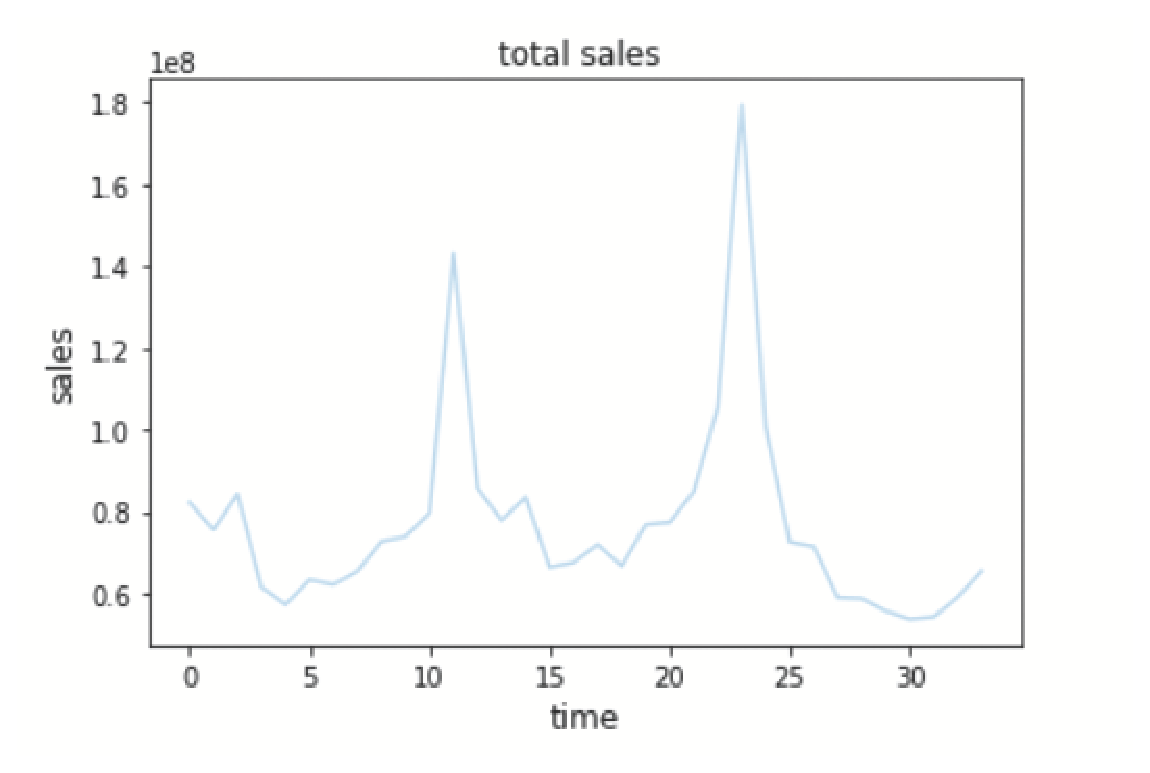
\includegraphics[width=4in]{p1}

\end{itemize}
\end{slide}


\begin{slide}{AUC }
\begin{itemize}
\item Validation AUC
\par
\includegraphics[width=4in]{AUC}
\par
Validation AUC = 0.805571412599524
\par
%\includegraphics[width=4in]{p2}
\end{itemize}
\end{slide}


\begin{slide}{Result}
\begin{enumerate}[type=1]%[label=\romani*)]
\item Probability
\par
\includegraphics[width=6in]{p013}
\end{enumerate}
\end{slide}


\section{Gaussian naive Bayes }
\begin{slide}{Statistical Functions}
\begin{itemize}[type=1]
\item Calculation of prior probability
\par
use Counter() maybe more convenient
\par
\item Avg and Std
\par
\item Calculate likelihood
\par
Using probability density function of Gaussian distribution to calculate likelihood and then multiply to get likelihood
We can get Raw data, trend data, periodic data, random variables
\par
\item Training model and get prediction
\par
The probabilities of each label are multiplied by the likelihood and then normalized to get the prob of each label.
\item AUC
\par
Validation AUC is 0.8051607443604657.
%\includegraphics[width=4in]{p3}
\end{itemize}
\end{slide}




\section{LinearRegression}
\begin{slide}{process}
\begin{itemize}
\item Merge test/train datasets
\par
\item Add more features
\par
Normalize the data,Standardization of normal distribution,then Square the value, cubic the value,Cumulative normal percentile,Normalize the data,again.Do linear regression,Write submission file
%\includegraphics[width=4in]{p5}
\par
AUC:  0.8025517936065763
\end{itemize}
\end{slide}


\section{ Catboost }
\begin{slide}{process}
\begin{itemize}
\item Feature Correlations
\par
\includegraphics[width=5in]{feature}
\item Get the features
Get the top 100 features,merge them and divide the training set and test set
\end{itemize}
\end{slide}
\begin{slide}{process}
\begin{itemize}
\item process data
\par
In catboost, you don't have to worry about this at all. You just need to tell the algorithm which features belong to category features, and it will help you deal with them automatically
\par
Finally, we feed the data to the algorithm and train it
\par
\includegraphics[width=5in]{cat}
\par
\item fit and prediction
\par
AUC: 0.80399151
\end{itemize}
\end{slide}
\section{Conclusion}
\begin{slide}{Compare}
\begin{itemize}
\item Naive Bayes
\par
AUC: 0.9055714
\item Gaussian naive Bayes
\par
AUC: 0.8051607
\item LinearRegression
\par
AUC: 0.8025517

\item Catboost
\par
AUC: 0.8039915

\end{itemize}
\end{slide}



\section{Thanks and Question}

\end{document}

\endinput
